\documentclass{article}
\usepackage{graphicx}
\usepackage[export]{adjustbox}
\usepackage[hidelinks=true,colorlinks=true]{hyperref}
\title{Safe Lane-Changing Solution For Automobiles}
\date{$17^{th}$ May 2017}
\author{Cherukuri Indu Susmitha - IMT2014011 \\ Meesala Vijaya Sindhu - IMT2014033 \\ Nikunj Gupta - IMT2014037 \\ Smit Patel - IMT2014051}
\begin{document}
	\maketitle
	\pagenumbering{roman}
	\section*{Abstract :}
	\subparagraph{}
	Safe Lane-Changing Solution is expected to be a mechanism which could aid in reducing the number of accidents due to sudden/unexpected lane changes by the drivers. Characteristics of the mechanism are as follows:
	\begin{itemize}
	\item If another vehicle is trying to overtake, the driver is warned to prevent a sudden lane change into the lane of the overtaking vehicle.
	\item If the driver is overtaking another vehicle, the driver is notified when he is far enough from the other vehicle to ensure a safe lane change.
	\item If the automobile is at rest and the driver wants to open its door from inside, the driver is restricted from doing so if there is an approaching vehicle on that side. Thus preventing collisions.  
	\end{itemize}		
	In this paper we describe our approach to the solution where the features from  the dataset are extracted using histogram of oriented gradients (hog), these features are used to train the SVM model to detect the automobiles and the output of the model is used to find the distance between the detected vehicles and the camera using triangular similarity and warn the driver when their is a possibility of accident.
	\section*{Introduction :}
	\subparagraph{}
	The major driving factor in support of implementation of this mechanism is the need to reduce number fatalities that take place around the globe either due to reckless lane changing by the drivers or due to their sudden actions which disrupt the normal flow of traffic in their surroundings. Some statistics which support this claim are as follows:
	\begin{itemize}
	\item A 2009 study by the American Automobile Association which attempted to identify behaviours associated with aggressive driving based on the data tracked by NHTSA’s Fatal Accident Report System (FARS) concluded that aggressive driving played a role in 56 percent of fatal crashes from 2003 through 2007, with erratic lane changing being one of the major factors followed by excessive speed.
	\item An analysis of the Chicago reported Bike crashes highlighted that there were 344 reported fatal dooring crashes reported in 2011, for a rate of 0.94 doorings per day. Also, Doorings made up 19.7\% of all reported bike crashes.
	\end{itemize}
	The proposed mechanism, if implemented on a large-scale across all automobiles has the potential to reduce these fatalities by a significant scale globally.\\
	\mbox{} \\
	There are many approaches that exist to detect vehicles and their relative position from your vehicle. One of the approaches is based on a stereo vision system. The input is the data from the vision system and from a positioning based system having a differential global positioning system (DGPS) and an inertial measurement unit (IMU). The most common approach to vehicle detection is to use active acoustic-based sensors. Optical sensors are also used mainly because they are cheap and because there are potential new applications such as lane detection, pedestrian detection, traffic sign recognition, etc. Initially, regions of interest (ROIs) are computed and then lane markings are detected, thus reducing the vehicle search area. If no lane markings are detected, a basic ROI corresponding to a straight road is used instead. Possible vehicle regions are selected using a combination of symmetries (vertical edges, horizontal edges, and gray level symmetries) and white hat and Canny features together with a non-maximum suppression procedure which removes overlapped candidates. Also, a second camera was added to obtain a more detailed description of the leading vehicles features. Stereo processing results in a dense disparity map which allows the 3D position, the time-to-Collision, the width, and the length of the vehicle to be estimated accurately. The camera pitch angle is estimated dynamically by means of the so-called virtual disparity map from which regions corresponding to the ground-plane can easily be removed.
	\section*{Description of Approach:}
	\subparagraph{}
	The project can basically be divided into two main parts:
	\begin{itemize}
	\item Firstly, detecting vehicles in the relevant ROI. For this we can collect relevant and precise dataset comprising of positive (images with car) and negative (images without cars) images. HOG features or SIFT/SURF features can be extracted from each of these images and using these features we can train KNN or perceptron or SVM model for classification or in our case car detection.
	\item Secondly, calculating the distance of the detected vehicle in the given frame. Calculating the distance can be done in various ways. We can use the concept of Triangular Similarity or Stereo Vision or Optical flow in images. Stereo vision uses two cameras placed next to each other to get a 3D view (similar to how humans are able to view in 3 dimensions). Triangular Similarity uses the concept of using the value of the focal length of the camera, pixel width of the object in the image and the known distance of the object in reality and then using these values to calculate the distance of the object in images. Optical flow uses the concept of calculating the distance travelled by the same object in various frames of a given video. This can be helpful to deduce the fact that whether the object is approaching or not, towards the leading vehicle.
	\end{itemize}
	Following is our approach to building the above mentioned mechanism.
	\begin{itemize}
	\item Firstly, for the part of \textbf{detection of car} in the image of the side-view camera we took the following approach:
	\begin{itemize}
	\item \textbf{Dataset Collection:} We collected a dataset of both positive and negative images which could aid us with sufficient features for the purpose of detection. We made sure that the dataset was distinct and thus covered most of the real-world scenarios while ensuring that the collected set of images always remained focussed to the end goal. The dataset we are presently using (Stanford car dataset) has 1000 positive (images with cars) and 1000 negative (images without cars like background, road, tree, etc.) image sets.
	\item \textbf{Feature Extraction: (Pre-Processing)} Once the dataset was successfully collected we extracted HOG (Histogram of Oriented Gradients) features from each of the images and stored them to a file along with their respective class labels. The histogram of oriented gradients (HOG) is a feature descriptor used in computer vision and image processing for the purpose of object detection. The technique counts occurrences of gradient orientation in localized portions of an image and is similar to that of edge orientation histograms, scale-invariant feature transform descriptors, and shape contexts, but differs in that it is computed on a dense grid of uniformly spaced cells and uses overlapping local contrast normalization for improved accuracy.
	\begin{center}
	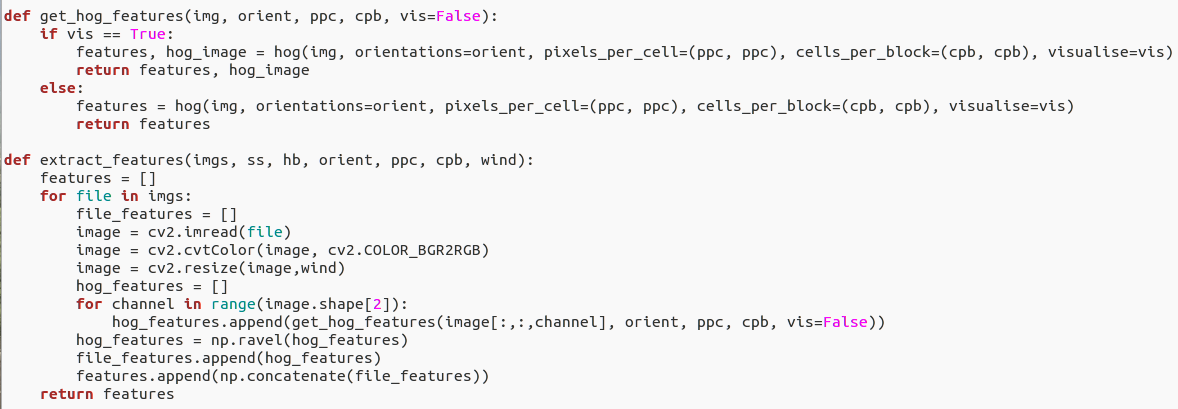
\includegraphics[max size={\textwidth}{\textheight}]{hog}
	\end{center}
	\item \textbf{Classifier Training: (Model Training)} The feature files thus created are used to train the SVM classifier which can then be used to predict the presence of the object in test images. SVM classifiers prevailed over the rest because its properties ensures that the chances of misclassification is minimal in most of the cases. The classifier parameters so obtained are then stored into a .pkl file for easy and immediate access while the process of detection on test images.
	\begin{center}
	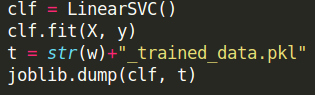
\includegraphics[scale=0.5]{SVM}
	\end{center}
	\item \textbf{Detection:} In order to detect cars in the test images, we implemented a sliding window mechanism which slides through the image in leaps of (100 * 100) window, extracting the features of each window, feeding it to the SVM classifier and checking if it has features similar to that of training images containing car. If so this window is marked to be a hot window. This mechanism is repeated with varying sizes of windows and at the end of the sliding window mechanism, the area of the image with the highest number of hot-window-intersections is determined and a rectangular bounding box is made around the same resulting in a rectangular region within the image which is supposed to have the highest probability of having a vehicle in it. The bounding box so obtained is the ROI which contains the car.
	\end{itemize}
	\item  Secondly, for \textbf{calculating the distance} of the detected vehicle in the given frame we took the following approach.
	\end{itemize}
	\section*{Future Work:}
	\subparagraph{}
	We are planning to collect more and better data, that is, more specific to our problem statement. The dataset which will be more specific to overtake detection will be only frontal vehicle images. Also, these images should be from a side-view mirrors angle. This can be achieved by taking a real time video of a road with some traffic from a camera kept at a stable position and angle.

Also, we have to figure out a better algorithm for car detection so that we can detect cars in real time. As of now, it takes a few seconds to detect a car in each frame of a video which needs to be reduced to at most 1 second. 

We are also planning to use stereo vision technology to calculate the distance of the vehicle from the leading vehicle. It should give better results. For this we will have to fix two cameras on each side of the car at some distance from each other and use the left and right image to find the accurate distance of the overtaking vehicle.
	\section*{References:}
	\subparagraph{}
\end{document}	